\chapter{Desarrollo Experimental}

\section{Experimento 1: Determinación del Factor de Potencia y Potencias Activa, Reactiva y Aparente}
En esta primera experiencia se analizó el comportamiento de una carga reactiva (tubo fluorescente con balasto inductivo)
conectada a la red eléctrica. Se implementó el circuito que se detalla en la figura del esquema del osciloscopio de la
consigna, utilizando una resistencia shunt $R_1 = 10\ohm$ para la medición indirecta de corriente (Canal 2 del
osciloscopio) y un divisor resistivo de tensión (Canal 1 del osciloscopio) compuesto por las resistencias de
$R_a = 86,7\kohm$ y $R_b = 9,88\kohm$.

La constante del divisor de tensión $k_{\text{div}}$ se define como:
\begin{equation}
    k_{\text{div}} = \frac{R_a + R_b}{R_b}
\end{equation}
Reemplazando por los valores medidos:
\[ k_{\text{div}} = \frac{86,7\kohm + 9,88\kohm}{9,88\kohm} = 9,7753 \]

Los valores medidos se detallan en la Tabla \ref{tab.mediciones:tp4_exp1}.

\begin{table}[!ht]
    \centering
    \resizebox{\textwidth}{!}{
    \begin{tabular}{|l|c|c|c|c|c|}
        \hline
        \textbf{Canal} & \textbf{Sensibilidad} & \textbf{$V_{\text{pap}}$} & \textbf{$V_{\text{ef}}$ (Osciloscopio)} & \textbf{$V_{\text{ef}}$ (Multímetro)} & \textbf{Incertidumbre (DMM)} \\ \hline
        Canal 1 (Tensión) & $10\V/\text{div}$ & $65,74\V$ & $23,24\V$ & $23,63\V$ & $\pm 0,27\V$ \\ \hline
        Canal 2 (Corriente) & $2\V/\text{div}$ & $11,05\V$ & $3,90\V$ & $3,60\V$ & $\pm 0,04\V$ \\ \hline
    \end{tabular}}
    \caption{Mediciones obtenidas en el Canal 1 y Canal 2 del osciloscopio y multímetro.}
    \label{tab.mediciones:tp4_exp1}
\end{table}

A partir de los valores medidos con el multímetro de referencia (UNI-T UT61D+), se calcularon los parámetros reales de
la línea de alimentación:
\begin{gather*}
    V_{\text{linea}} = V_{C1,\text{ef}} \cdot k_{\text{div}} = 23,63\V \cdot 9,7753 = 230,99\V \approx 231\V \\
    I_{\text{linea}} = \frac{V_{C2,\text{ef}}}{R_1} = \frac{3,60\V}{10\ohm} = 0,36\A
\end{gather*}

Si se realiza el cálculo a partir de los datos indicados por el osciloscopio:
\begin{gather*}
    V_{\text{linea, osc}} = 23,24\V \cdot 9,7753 = 227,18\V \\
    I_{\text{linea, osc}} = \frac{3,90\V}{10\ohm} = 0,39\A
\end{gather*}

Para medir el desfasaje se utilizó la figura de Lissajous mostrada en el osciloscopio en modo X-Y. La imagen elíptica
obtenida se presenta en la foto de laboratorio en la figura \ref{fig.osc:v_xy}. Las dimensiones de la elipse sobre la
grilla del osciloscopio fueron:
\begin{itemize}
    \item Intersección de la elipse con el eje Y ($A$): $5,2\text{ divisiones}$.
    \item Amplitud máxima en el eje Y ($B$): $5,5\text{ divisiones}$.
\end{itemize}

El desfasaje $\phi$ se calcula de forma indirecta mediante la relación de amplitudes:
\begin{equation}
    \sin\phi = \frac{A}{B}
\end{equation}
Sustituyendo por los valores leídos:
\[ \sin\phi = \frac{5,2}{5,5} = 0,9455 \]

A partir de esta relación se deducen el ángulo y sus parámetros asociados:
\begin{gather*}
    \phi = \arcsin(0,9455) \approx 71^\circ \\
    \cos\phi = 0,325 \\
    \tan\phi = 2,902
\end{gather*}

Con los valores calculados de tensión de línea ($227,15\V$ según la aproximación manuscrita) e intensidad de línea
($0,36\A$), se determinan las potencias reactiva, activa y aparente de la carga inductiva:
\begin{itemize}
    \item \textbf{Potencia Aparente ($S$):}
          \begin{equation}
              S = V_{\text{linea}} \cdot I_{\text{linea}}
          \end{equation}
          Reemplazando por los valores correspondientes:
          \[ S = 227,15\V \cdot 0,36\A = 81,77\text{ VA} \]
    \item \textbf{Potencia Activa ($P$):}
          \begin{equation}
              P = S \cdot \cos\phi
          \end{equation}
          Reemplazando por los valores correspondientes:
          \[ P = 81,77\text{ VA} \cdot 0,325 = 26,57\W \]
    \item \textbf{Potencia Reactiva ($Q$):}
          \begin{equation}
              Q = S \cdot \sin\phi
          \end{equation}
          Reemplazando por los valores correspondientes:
          \[ Q = 81,77\text{ VA} \cdot 0,945 = 77,27\text{ VAR} \]
\end{itemize}

\begin{figure}[!ht]
    \centering
    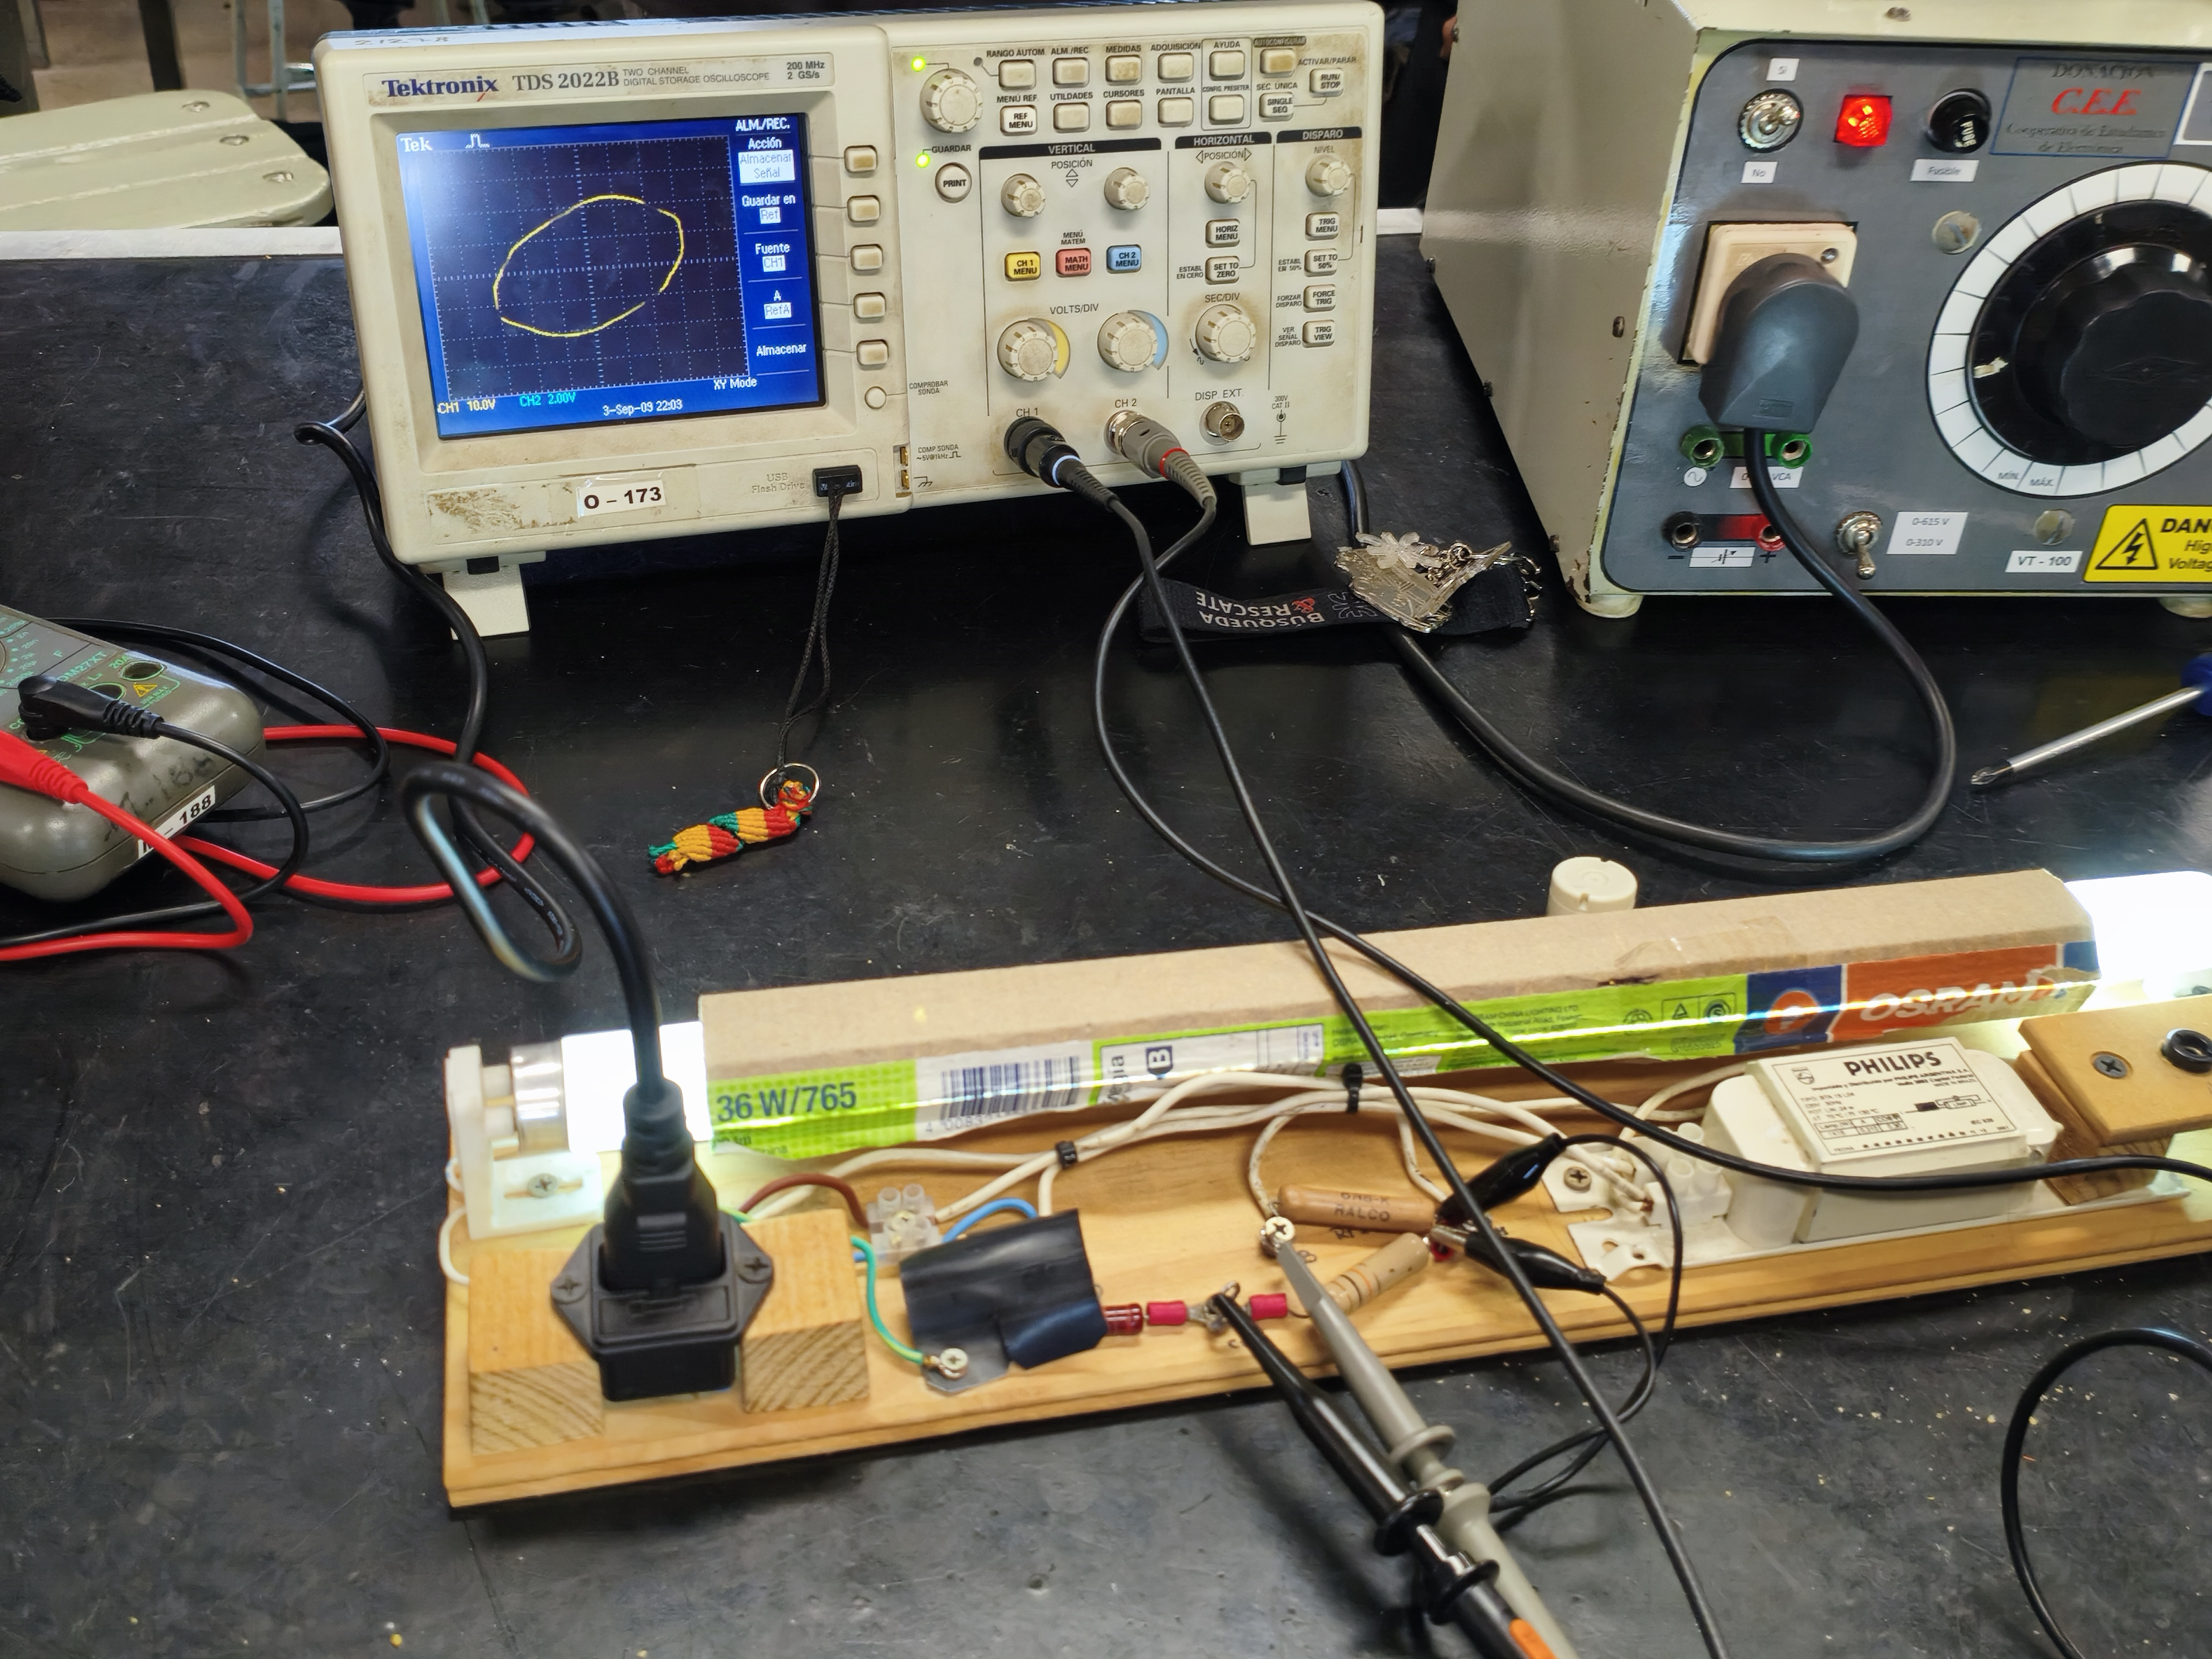
\includegraphics[height=\fotoheight]{pictures/osc_v_xy.jpg}
    \caption{Elipse de Lissajous en modo X-Y para la determinación del desfasaje entre tensión y corriente.}
    \label{fig.osc:v_xy}
\end{figure}


\section{Experimento 2: Compensación y Corrección del Factor de Potencia}
Para corregir el bajo factor de potencia de la lámpara fluorescente ($\cos\phi = 0,325$), se debe conectar un
capacitor en paralelo con la carga. El valor de capacidad necesario para realizar la compensación ideal ($\cos\phi_f = 1$)
se calcula como:
\begin{equation}
    C = \frac{P \cdot \tan\phi}{V_{\text{linea}}^2 \cdot \omega}
\end{equation}
Sustituyendo los valores de ensayo:
\[ C = \frac{26,57\W \cdot 2,902}{(227,15\V)^2 \cdot 2\pi \cdot 50\Hz} \approx 4,756\uF \]

Utilizando el medidor LCR digital Agilent U1733C, se midió el valor real del capacitor del laboratorio, obteniendo
una capacidad de $C_{\text{medida}} = 4,906\uF$ con un ángulo de fase de $-88,1^\circ$. La medición correspondiente se
ilustra en la figura \ref{fig.lcr:capacitor}.

\begin{figure}[!ht]
    \centering
    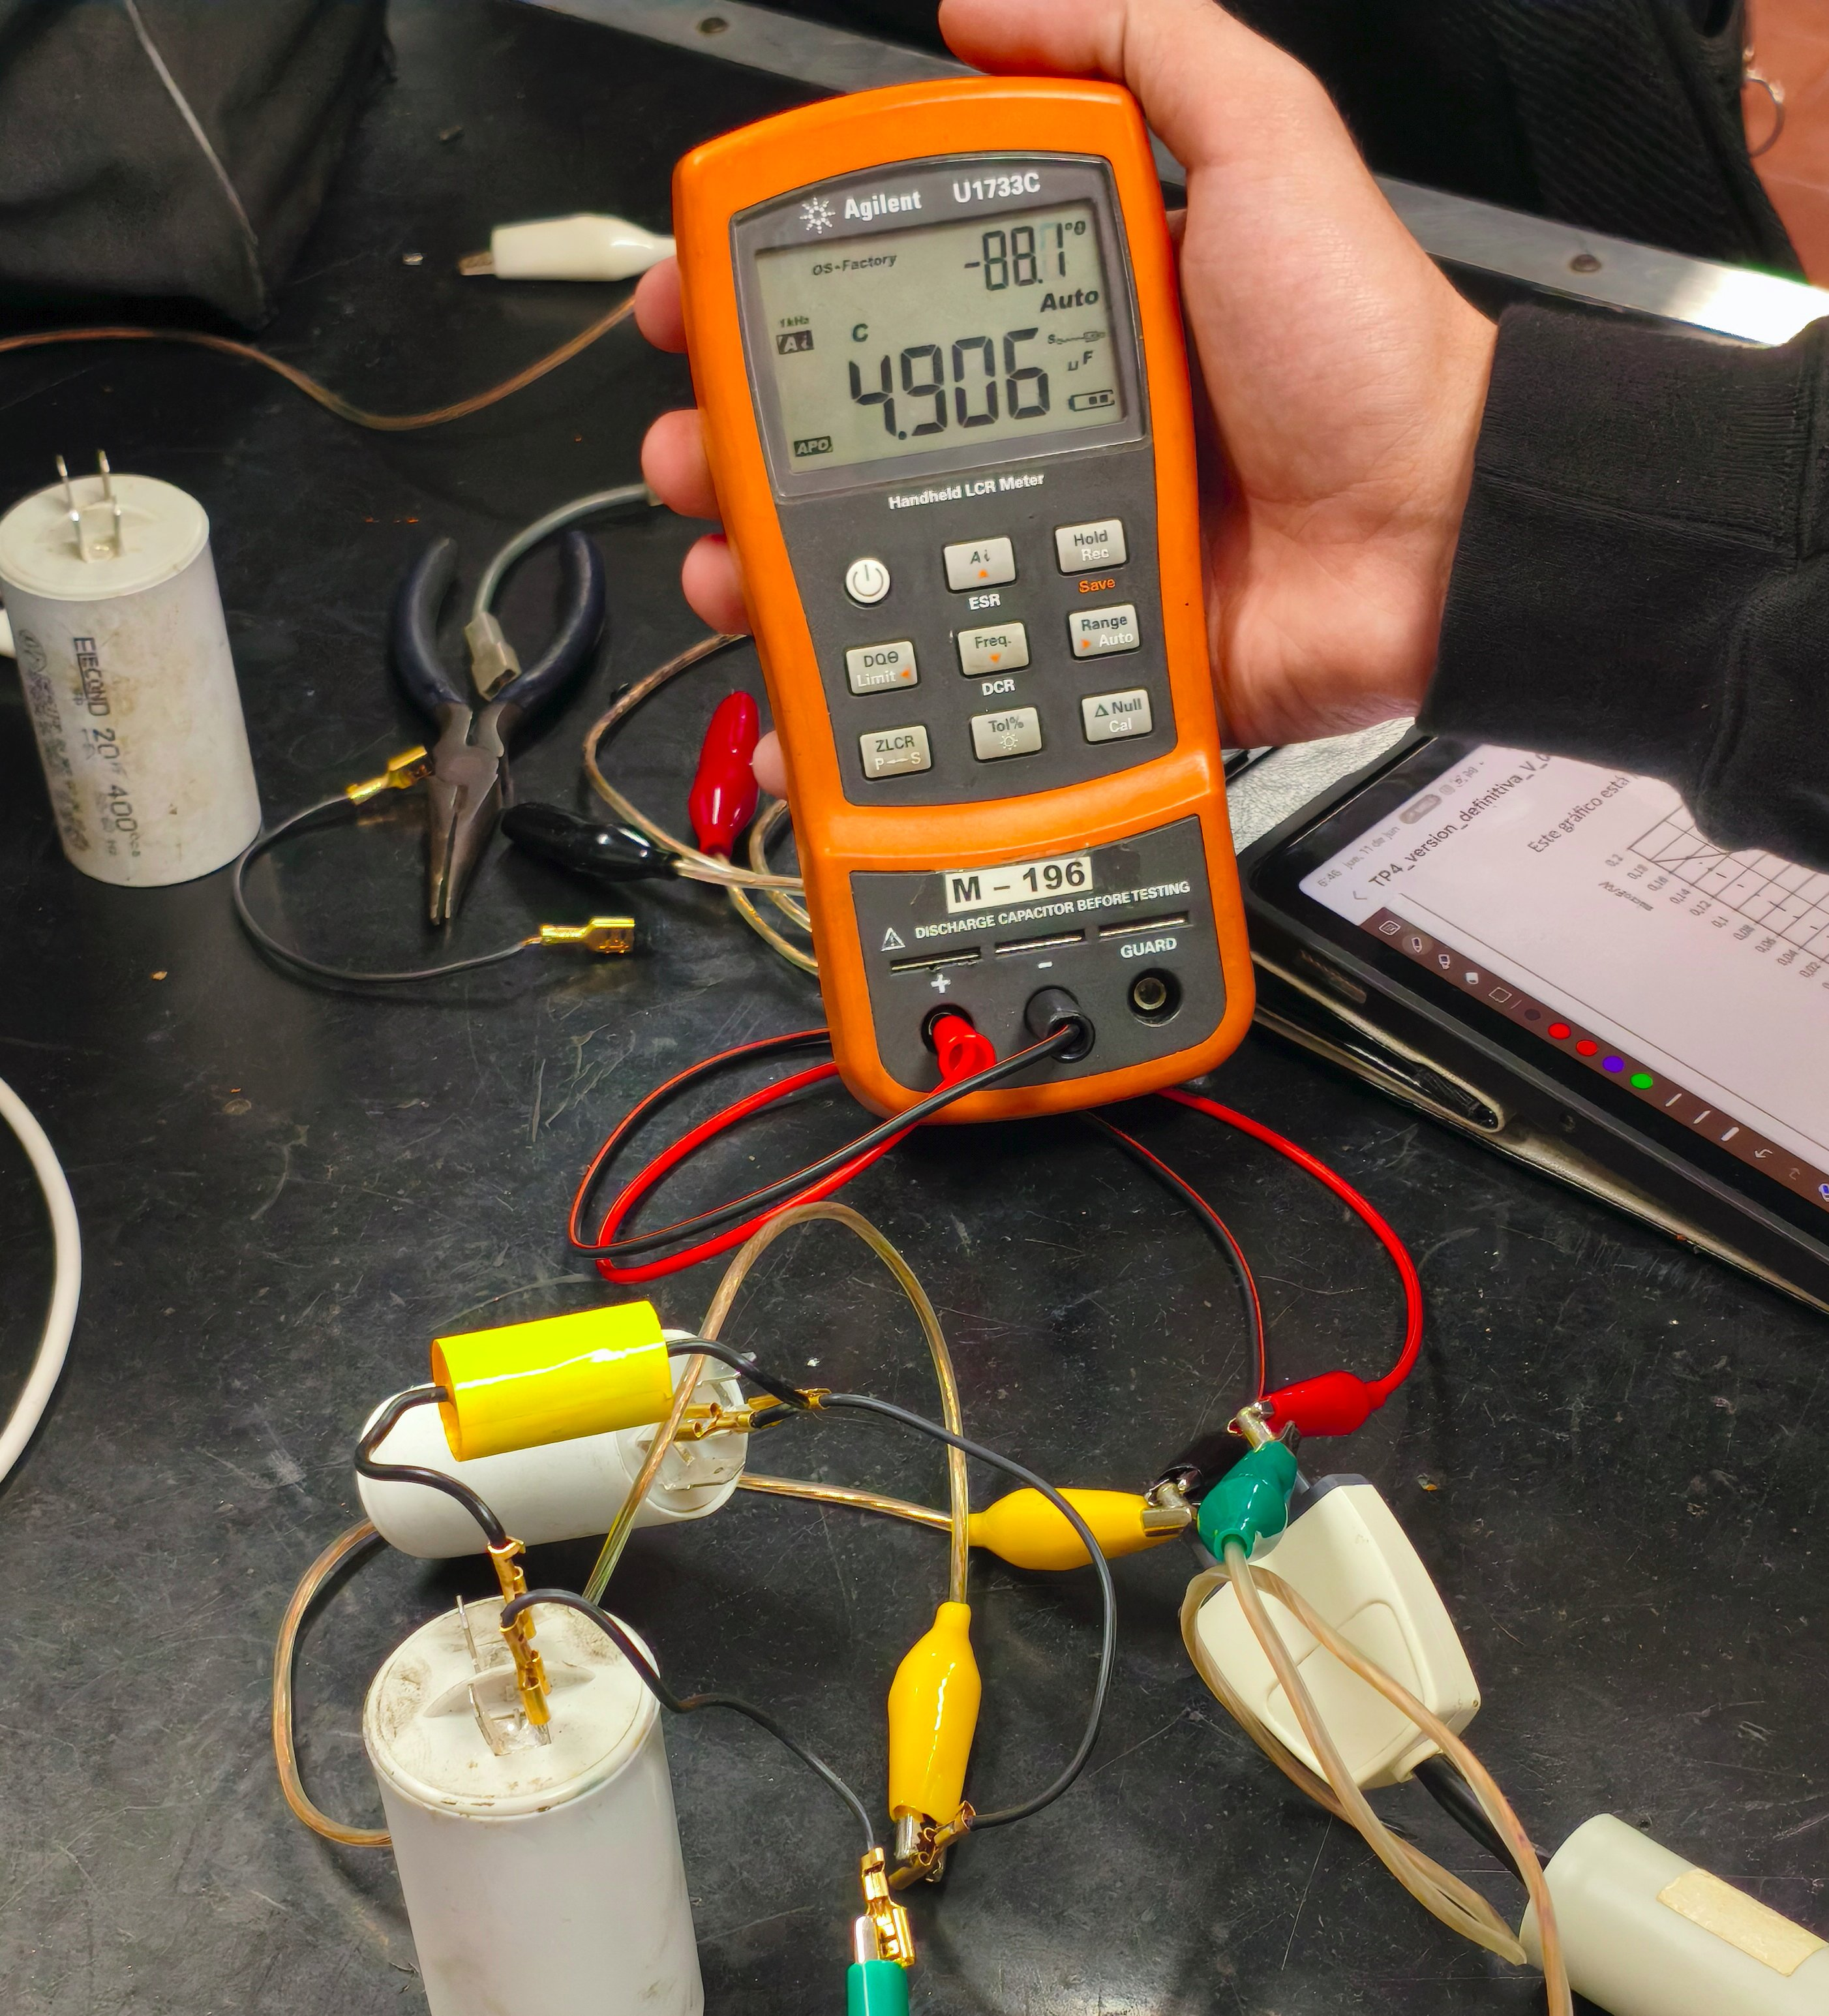
\includegraphics[height=\fotoheight]{pictures/lcr_meter_cap.jpg}
    \caption{Medición de la capacidad real en el LCR digital Agilent U1733C.}
    \label{fig.lcr:capacitor}
\end{figure}

Al conectar el capacitor de corrección en paralelo, se obtuvieron las siguientes lecturas del osciloscopio en el
dominio del tiempo:
\begin{gather*}
    V_{C1,\text{ef}} = 23,26\V \implies V_{\text{linea}} = 227,37\V \\
    I_{\text{linea}} = \frac{1,348\V}{10\ohm} = 0,1348\A
\end{gather*}

Con estas lecturas se calcula la nueva potencia aparente tomada de la línea:
\[ S_{\text{corr}} = V_{\text{linea}} \cdot I_{\text{linea}} = 227,37\V \cdot 0,1348\A = 30,65\text{ VA} \]

Al comparar con la situación previa a la compensación, se comprueba una gran reducción de la corriente tomada de la
red (de $0,36\A$ a $0,1348\A$) y, por ende, de la potencia aparente (de $81,77\text{ VA}$ a $30,65\text{ VA}$), lo que representa
una disminución del $62,5\%$. Las formas de onda corregidas en pantalla se presentan en la figura \ref{fig.osc:corrected}.

\begin{figure}[!ht]
    \centering
    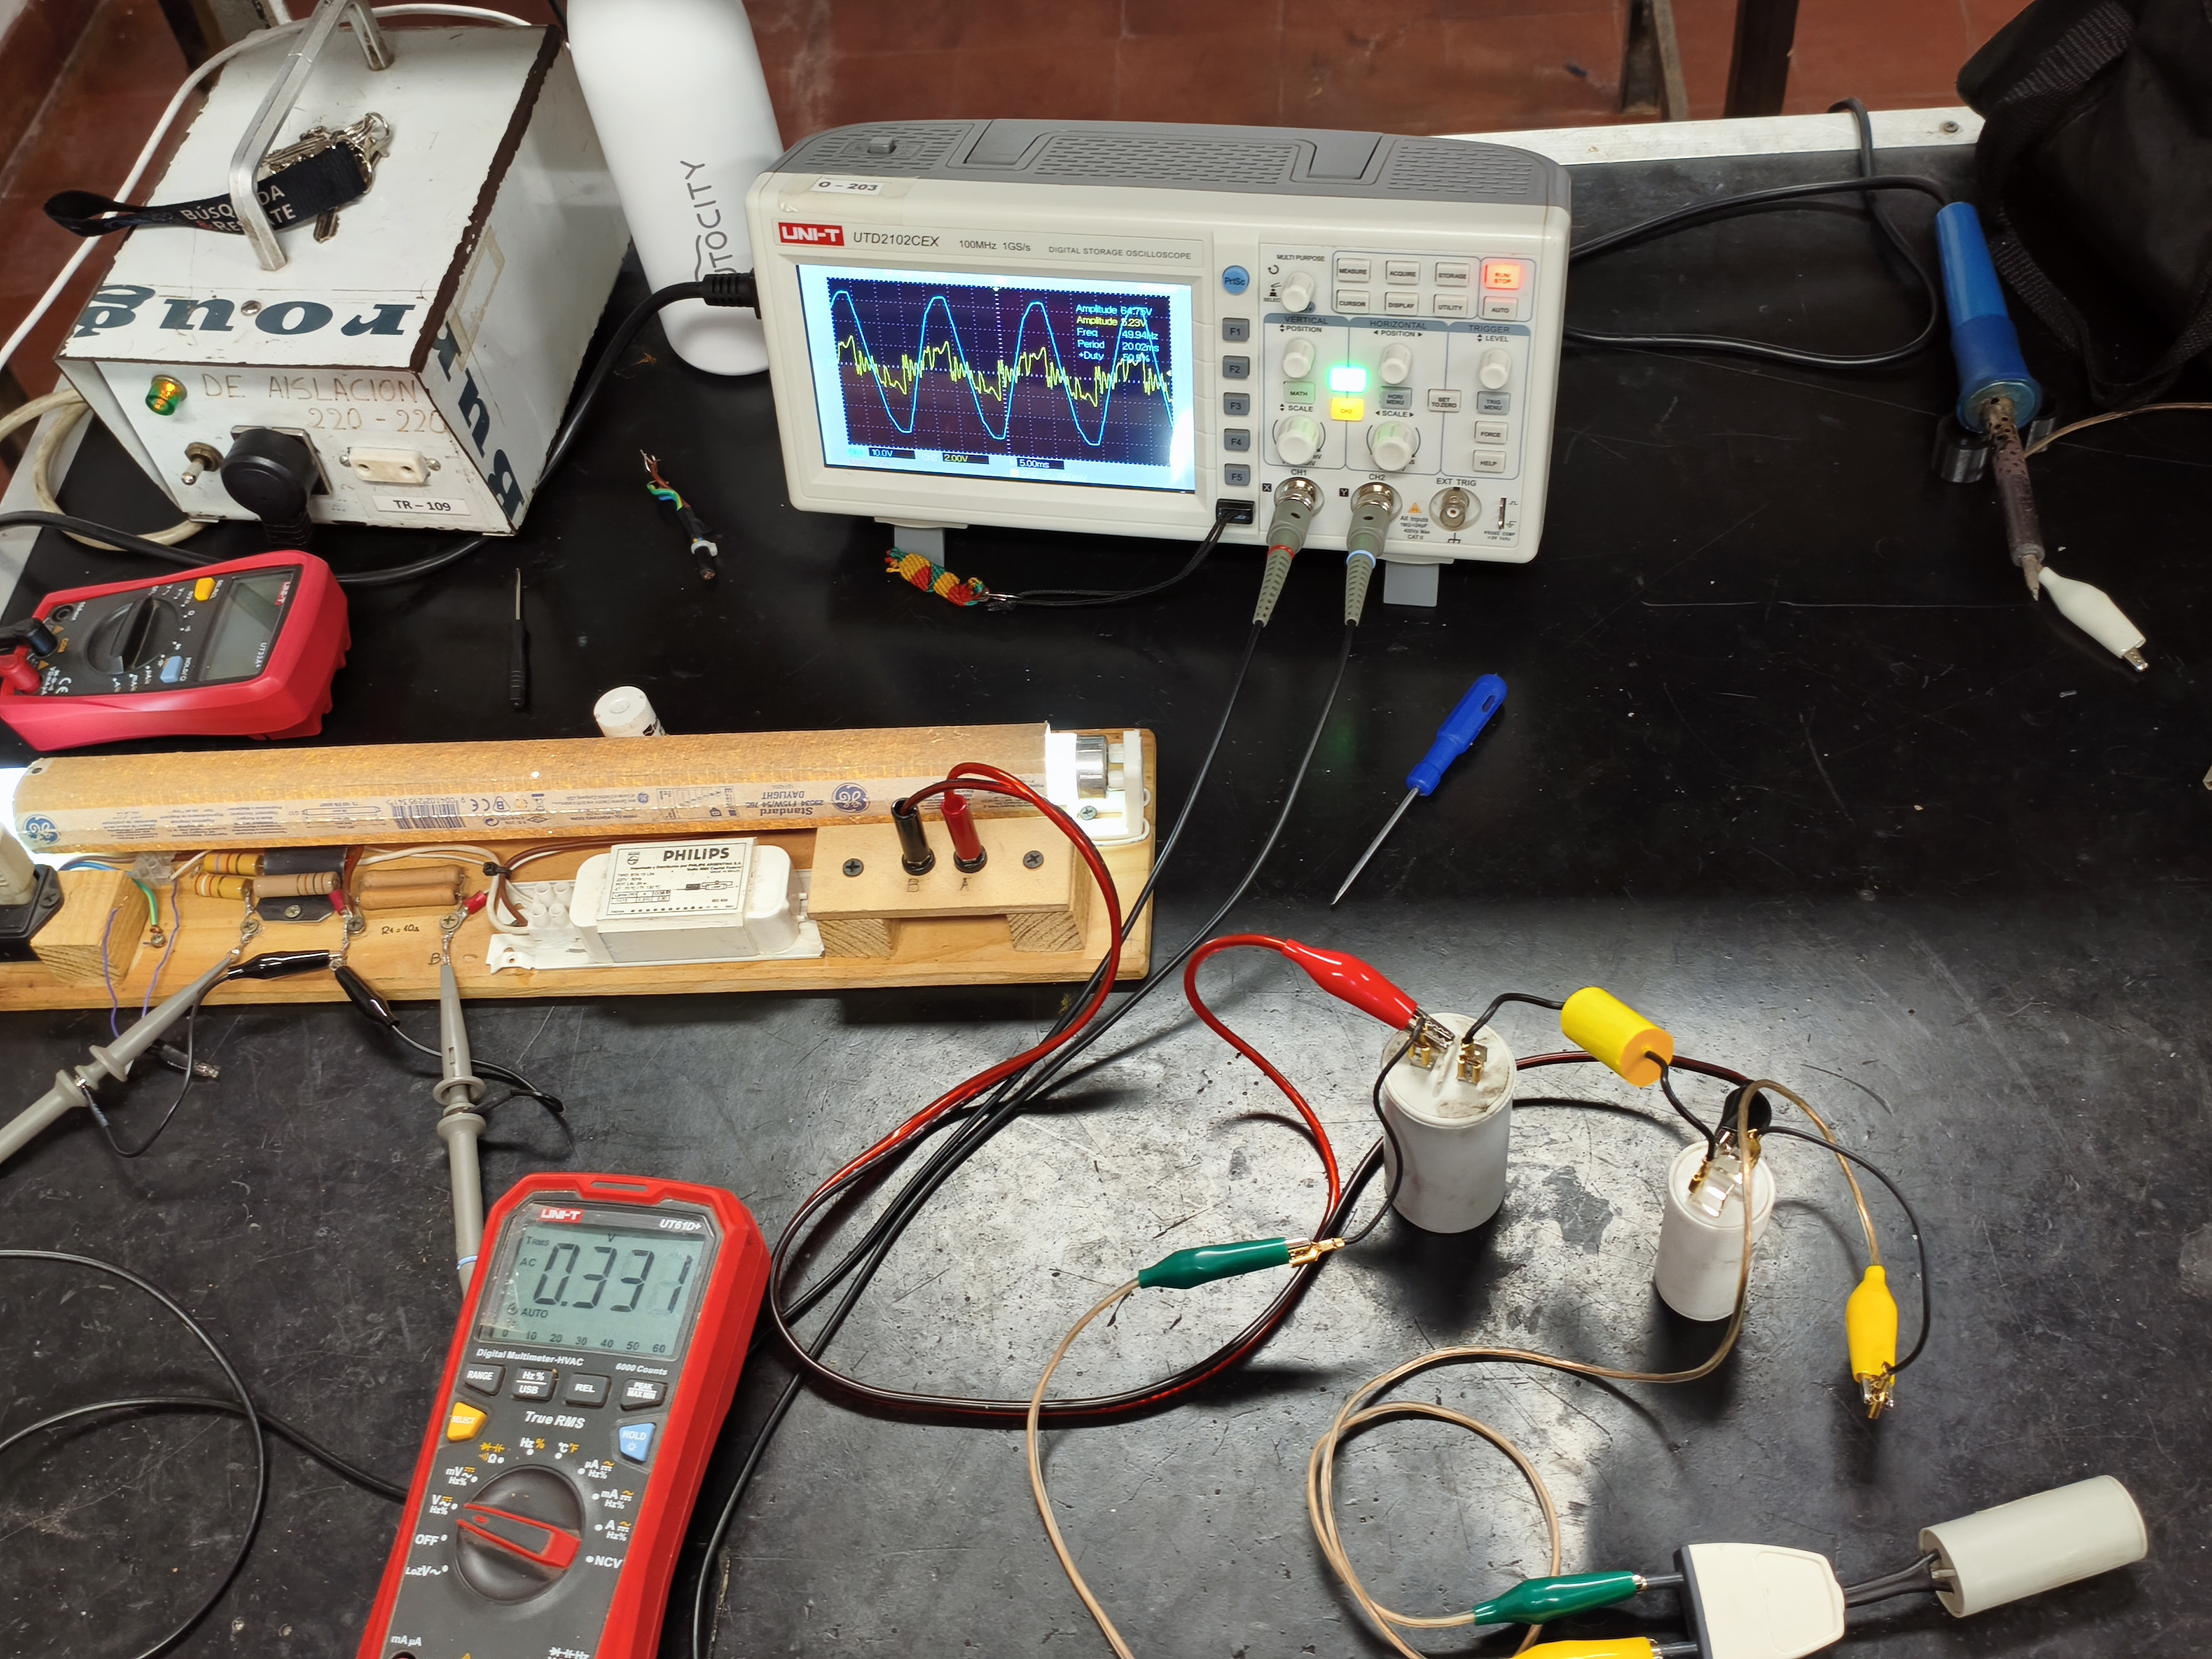
\includegraphics[height=\fotoheight]{pictures/osc_v_corrected.jpg}
    \caption{Tensión (onda senoidal definida) y corriente corregida del circuito con capacitor en paralelo.}
    \label{fig.osc:corrected}
\end{figure}


\section{Experimento 3: Medición de Formas de Onda no Sinusoidales (Cuadrada y Triangular)}
Se conectó un generador de funciones configurado para suministrar señales de $50\Hz$ y amplitud de $5\text{ V}_{\text{pp}}$.
Se midió la tensión de salida utilizando un voltímetro True RMS (UNI-T UT61D+) y un voltímetro de respuesta al valor medio
calibrado para señales sinusoidales (UNI-T UT33A+). Ambos instrumentos se colocaron en el rango de $4\V$ de corriente
alterna. Los resultados obtenidos se muestran en la Tabla \ref{tab.ondas:tp4_exp3}.

\begin{table}[!ht]
    \centering
    \resizebox{\textwidth}{!}{
    \begin{tabular}{|l|c|c|c|}
        \hline
        \textbf{Tipo de Onda} & \textbf{Lectura True RMS ($V_{\text{RMS}}$)} & \textbf{Lectura Valor Medio ($V_{\text{medio}}$)} & \textbf{Error Relativo ($e\%$)} \\ \hline
        Cuadrada ($50\Hz$, $5\text{ V}_{\text{pp}}$) & $2,486\V$ & $2,500\V$ & $+0,56\%$ \\ \hline
        Triangular ($50\Hz$, $5\text{ V}_{\text{pp}}$) & $1,421\V$ & $1,424\V$ & $+0,21\%$ \\ \hline
    \end{tabular}}
    \caption{Comparativa de mediciones para ondas cuadrada y triangular.}
    \label{tab.ondas:tp4_exp3}
\end{table}

El error relativo porcentual se calcula como:
\begin{equation}
    e\% = \frac{V_{\text{medio}} - V_{\text{RMS}}}{V_{\text{RMS}}} \cdot 100
\end{equation}

Las fotos del instrumental durante la medición de la onda cuadrada y triangular se pueden ver en las figuras
\ref{fig.dmm:square} y \ref{fig.dmm:triangular}.

\begin{figure}[!ht]
    \centering
    \begin{subfigure}[t]{0.56\textwidth}
        \centering
        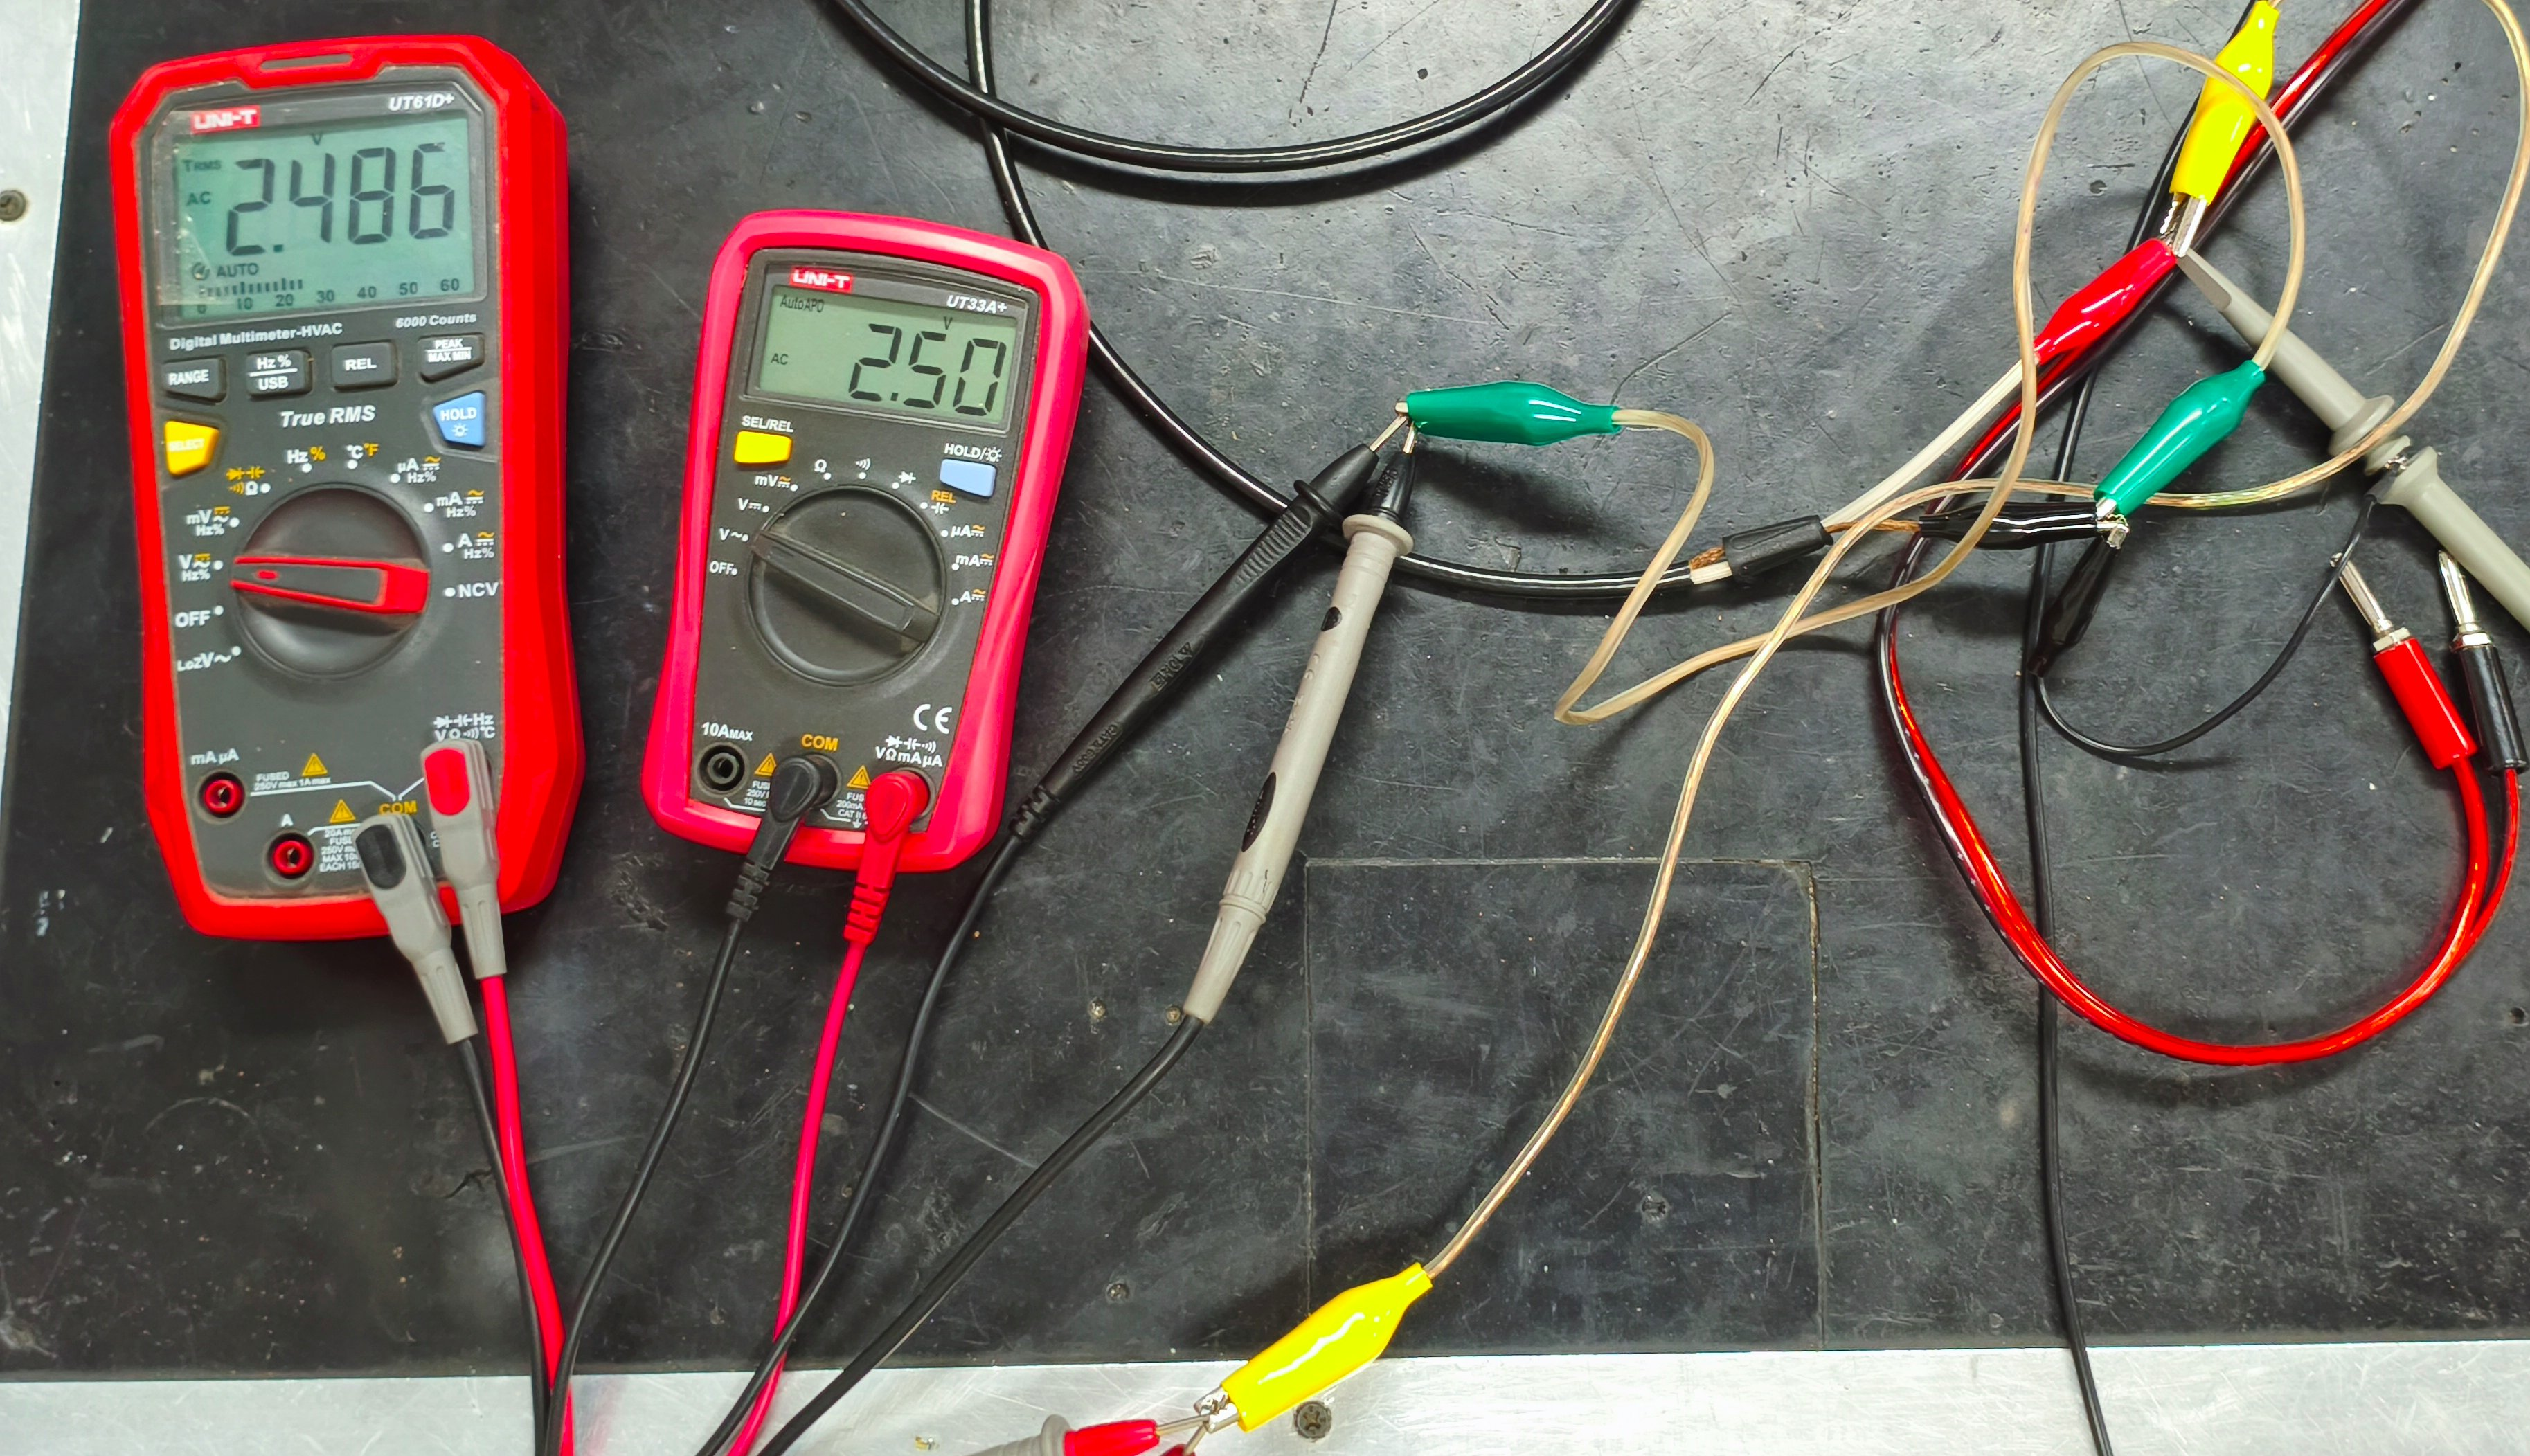
\includegraphics[height=\fotoheight]{pictures/square_wave_dmm.jpg}
        \caption{Medición de onda cuadrada (Setup).}
        \label{fig.dmm:square}
    \end{subfigure}
    \hfill
    \begin{subfigure}[t]{0.40\textwidth}
        \centering
        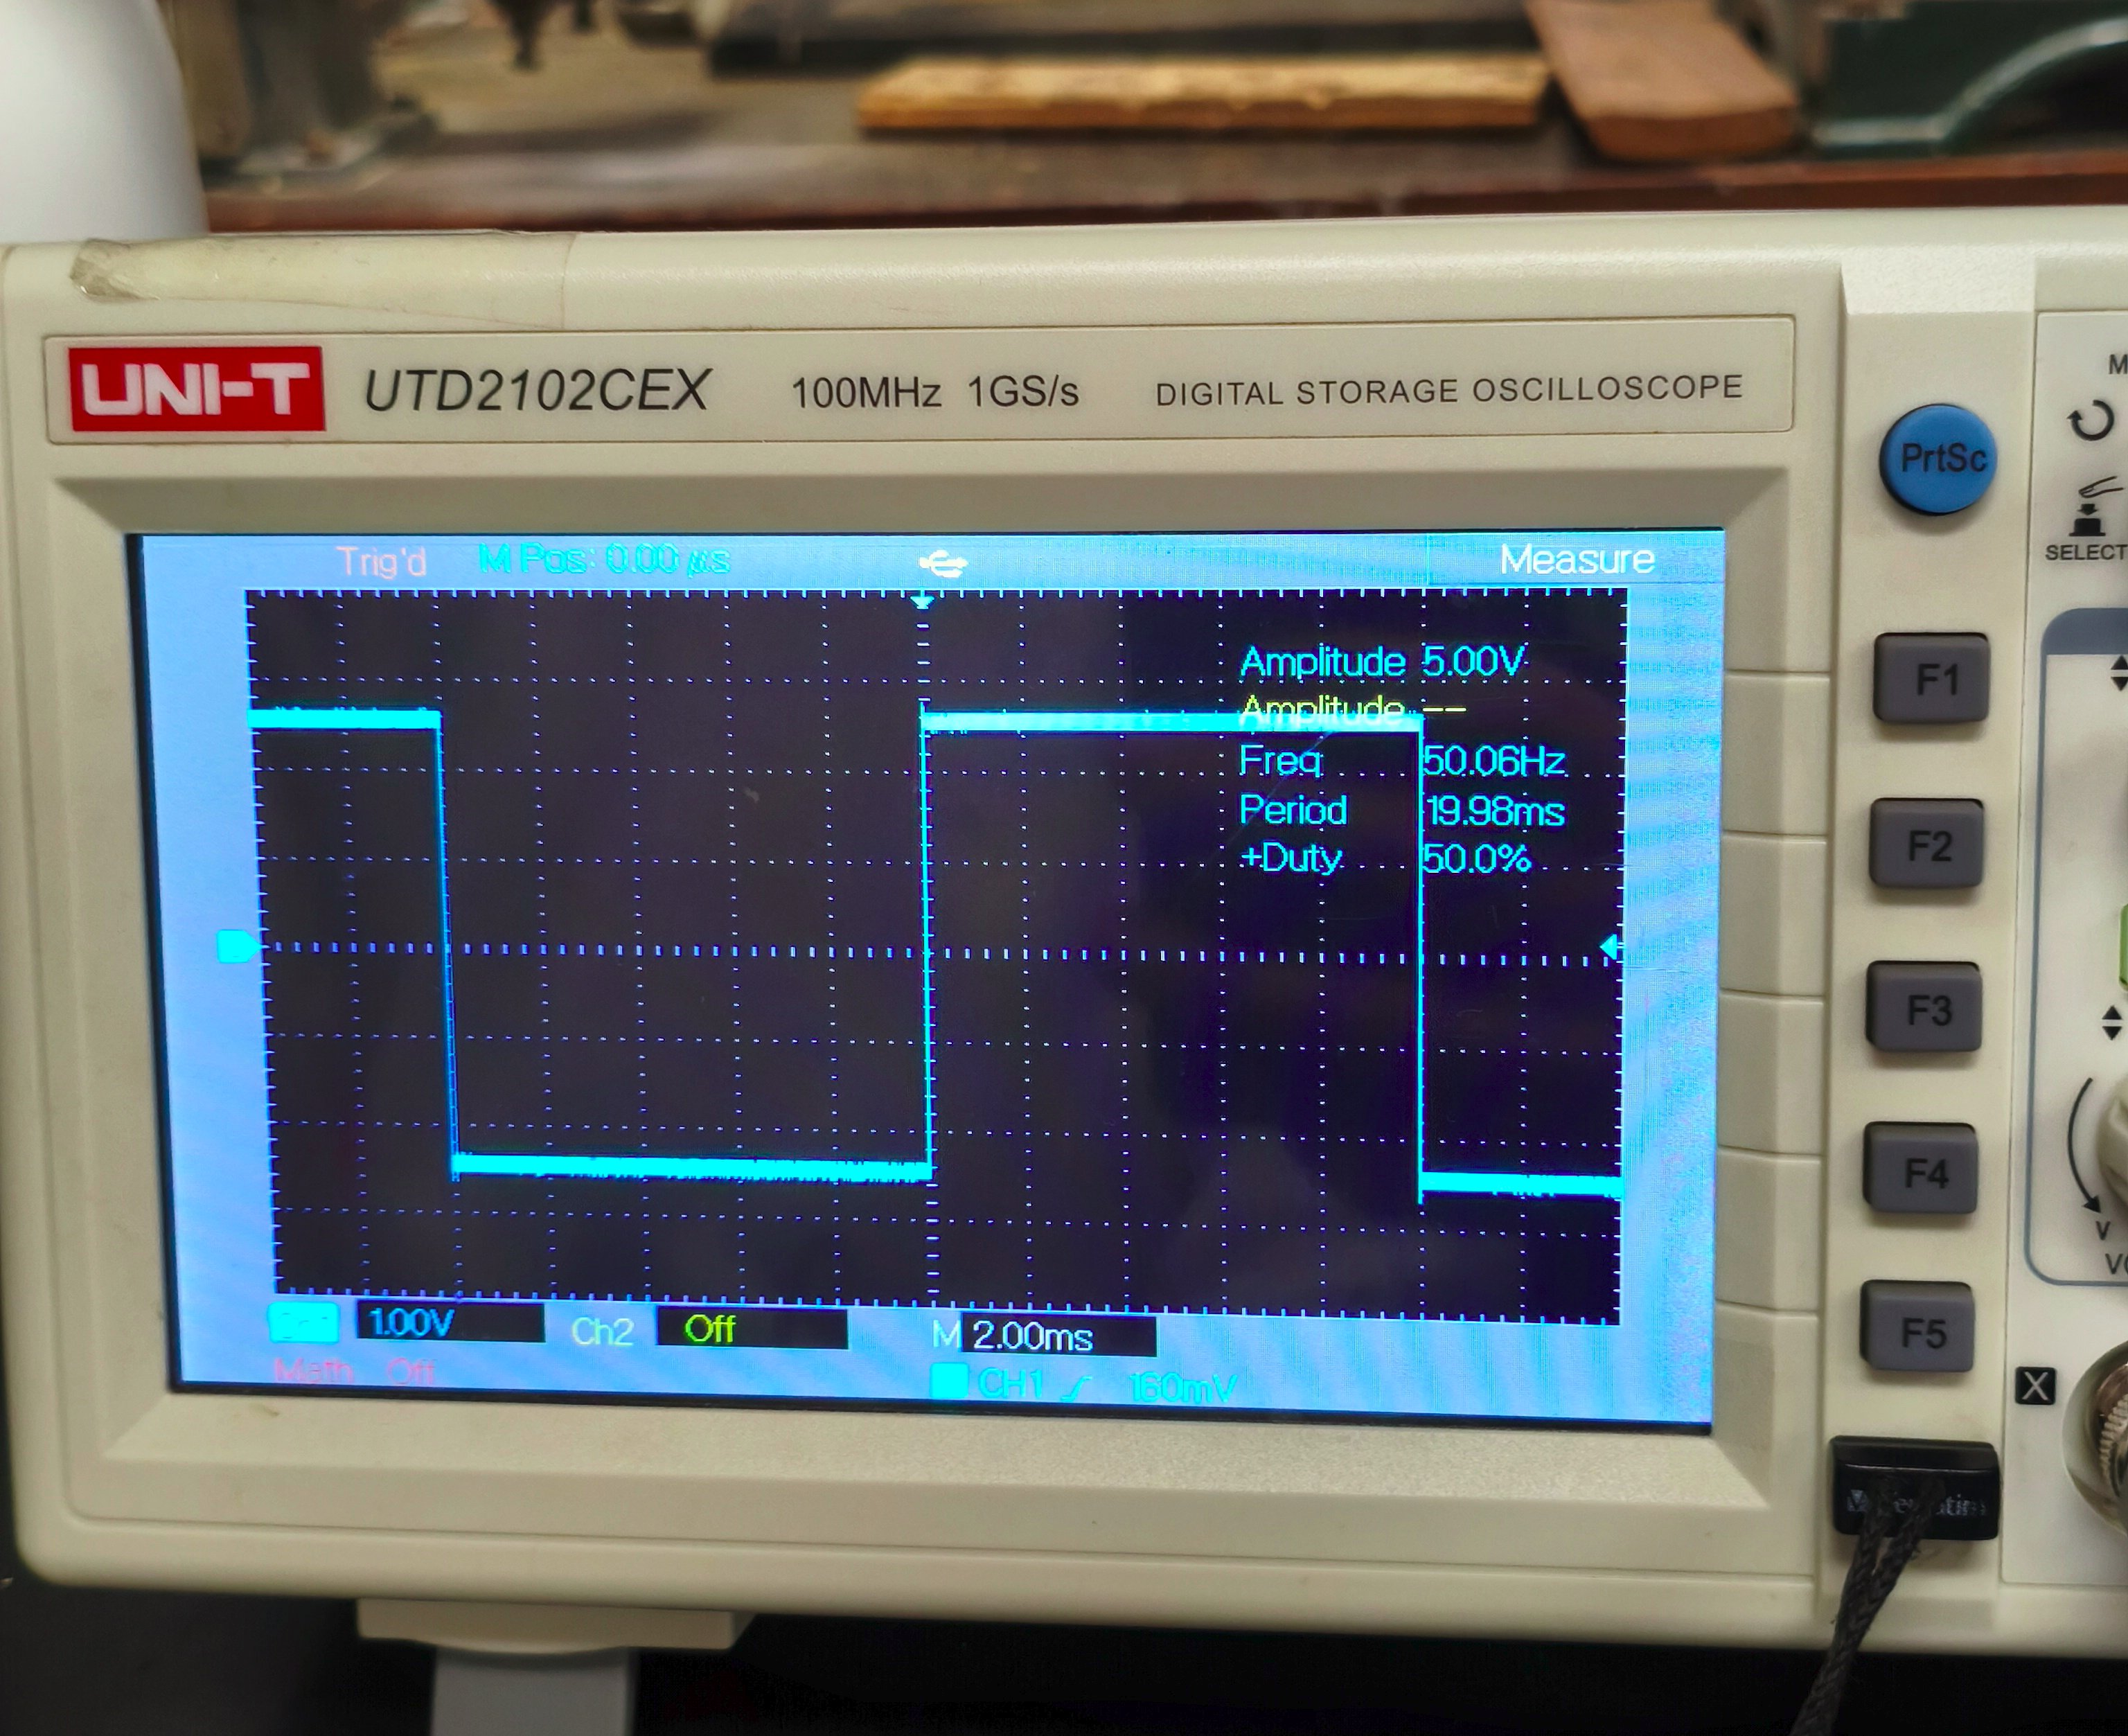
\includegraphics[height=\fotoheight]{pictures/square_wave_dmm_2.jpg}
        \caption{Medición de onda cuadrada (Osciloscopio).}
        \label{fig.dmm:triangular}
    \end{subfigure}
    \caption{Lecturas en multímetros para señales no sinusoidales de $5\text{ V}_{\text{pp}}$.}
\end{figure}


\section{Experimento 4: Control de Ángulo de Conducción por Triac (Dimmer)}
Se alimentó un circuito regulador dimmerizador por corte de fase con una tensión de entrada nominal $V_i = 231,9\V$.
Variando el ángulo de retardo de disparo $\alpha$, se midió la tensión eficaz de salida $V_o$ sobre una lámpara
incandescente utilizando ambos multímetros. Se calculó la relación de transferencia de tensión $V_o/V_i$ y las
incertidumbres absolutas asociadas a las lecturas según las especificaciones técnicas de exactitud de los manuales de
usuario. Los valores medidos y calculados se resumen en la Tabla \ref{tab.dimmer:tp4_exp4}.

\begin{table}[!ht]
    \centering
    \resizebox{\textwidth}{!}{
    \begin{tabular}{|c|c|c|c|c|c|c|}
        \hline
        \textbf{Ángulo de Retardo ($\alpha$)} & \textbf{$V_{o1}$ True RMS} & \textbf{$V_{o2}$ Valor Medio} & \textbf{$V_{o1}/V_i$} & \textbf{$V_{o2}/V_i$} & \textbf{Incertidumbre $V_{o1}$} & \textbf{Incertidumbre $V_{o2}$} \\ \hline
        $0^\circ$ & -- & -- & -- & -- & -- & -- \\ \hline
        $30^\circ$ & $224,3\V$ & $225,0\V$ & $0,967$ & $0,970$ & $\pm 2,54\V$ & $\pm 3,00\V$ \\ \hline
        $60^\circ$ & $211,2\V$ & $212,0\V$ & $0,911$ & $0,914$ & $\pm 2,41\V$ & $\pm 2,84\V$ \\ \hline
        $90^\circ$ & $175,9\V$ & $176,5\V$ & $0,759$ & $0,761$ & $\pm 2,06\V$ & $\pm 2,42\V$ \\ \hline
        $120^\circ$ & $124,8\V$ & $125,2\V$ & $0,538$ & $0,540$ & $\pm 1,55\V$ & $\pm 1,80\V$ \\ \hline
        $150^\circ$ & $45,26\V$ & $52,90\V$ & $0,195$ & $0,228$ & $\pm 0,48\V$ & $\pm 0,93\V$ \\ \hline
        $180^\circ$ & $0,20\V$ & $0,20\V$ & $0,001$ & $0,001$ & $\pm 0,01\V$ & $\pm 0,01\V$ \\ \hline
    \end{tabular}}
    \caption{Tensión eficaz de salida en función de la fase de retardo de disparo del Triac.}
    \label{tab.dimmer:tp4_exp4}
\end{table}

Las fórmulas utilizadas para el cálculo de las incertidumbres absolutas ($\Delta V$) son:
\begin{gather}
    \Delta V_{o1} = \pm (1,0\% \cdot V_{o1} + 3 \cdot \text{resolución}) \quad \text{[UT61D+ True RMS]} \\
    \Delta V_{o2} = \pm (1,2\% \cdot V_{o2} + 3 \cdot \text{resolución}) \quad \text{[UT33A+ Valor Medio]}
\end{gather}


\section{Experimento 5: Análisis de Potencia con Carga Dimmerizada}
Se ajustó el ángulo de conducción del dimmer para obtener una tensión eficaz de aproximadamente $110\V$ sobre la carga
($V_{\text{RMS}} = 110,6\V$ en el multímetro True RMS, y $110,8\V$ en el de valor medio). Se conectó el medidor de consumo y
potencia digital en la entrada del sistema y se registraron los siguientes parámetros:
\begin{itemize}
    \item Corriente total de línea ($I$): $0,138\A$.
    \item Tensión de línea ($V_i$): $218,1\V$ (según la lectura de tensión del medidor).
    \item Potencia activa medida ($P$): $12,0\W$.
    \item Factor de potencia indicado ($\text{PF}$): $0,43$.
\end{itemize}

El montaje del dimmer con la lámpara y el medidor de consumo se puede ver en la figura \ref{fig.dimmer:setup}.

\begin{figure}[!ht]
    \centering
    \begin{subfigure}[t]{0.45\textwidth}
        \centering
        \includegraphics[height=\fotoheight]{pictures/dimmer_setup_close.jpg}
        \caption{Conexiones y circuito dimmer.}
    \end{subfigure}
    \hspace{1.5cm}
    \begin{subfigure}[t]{0.25\textwidth}
        \centering
        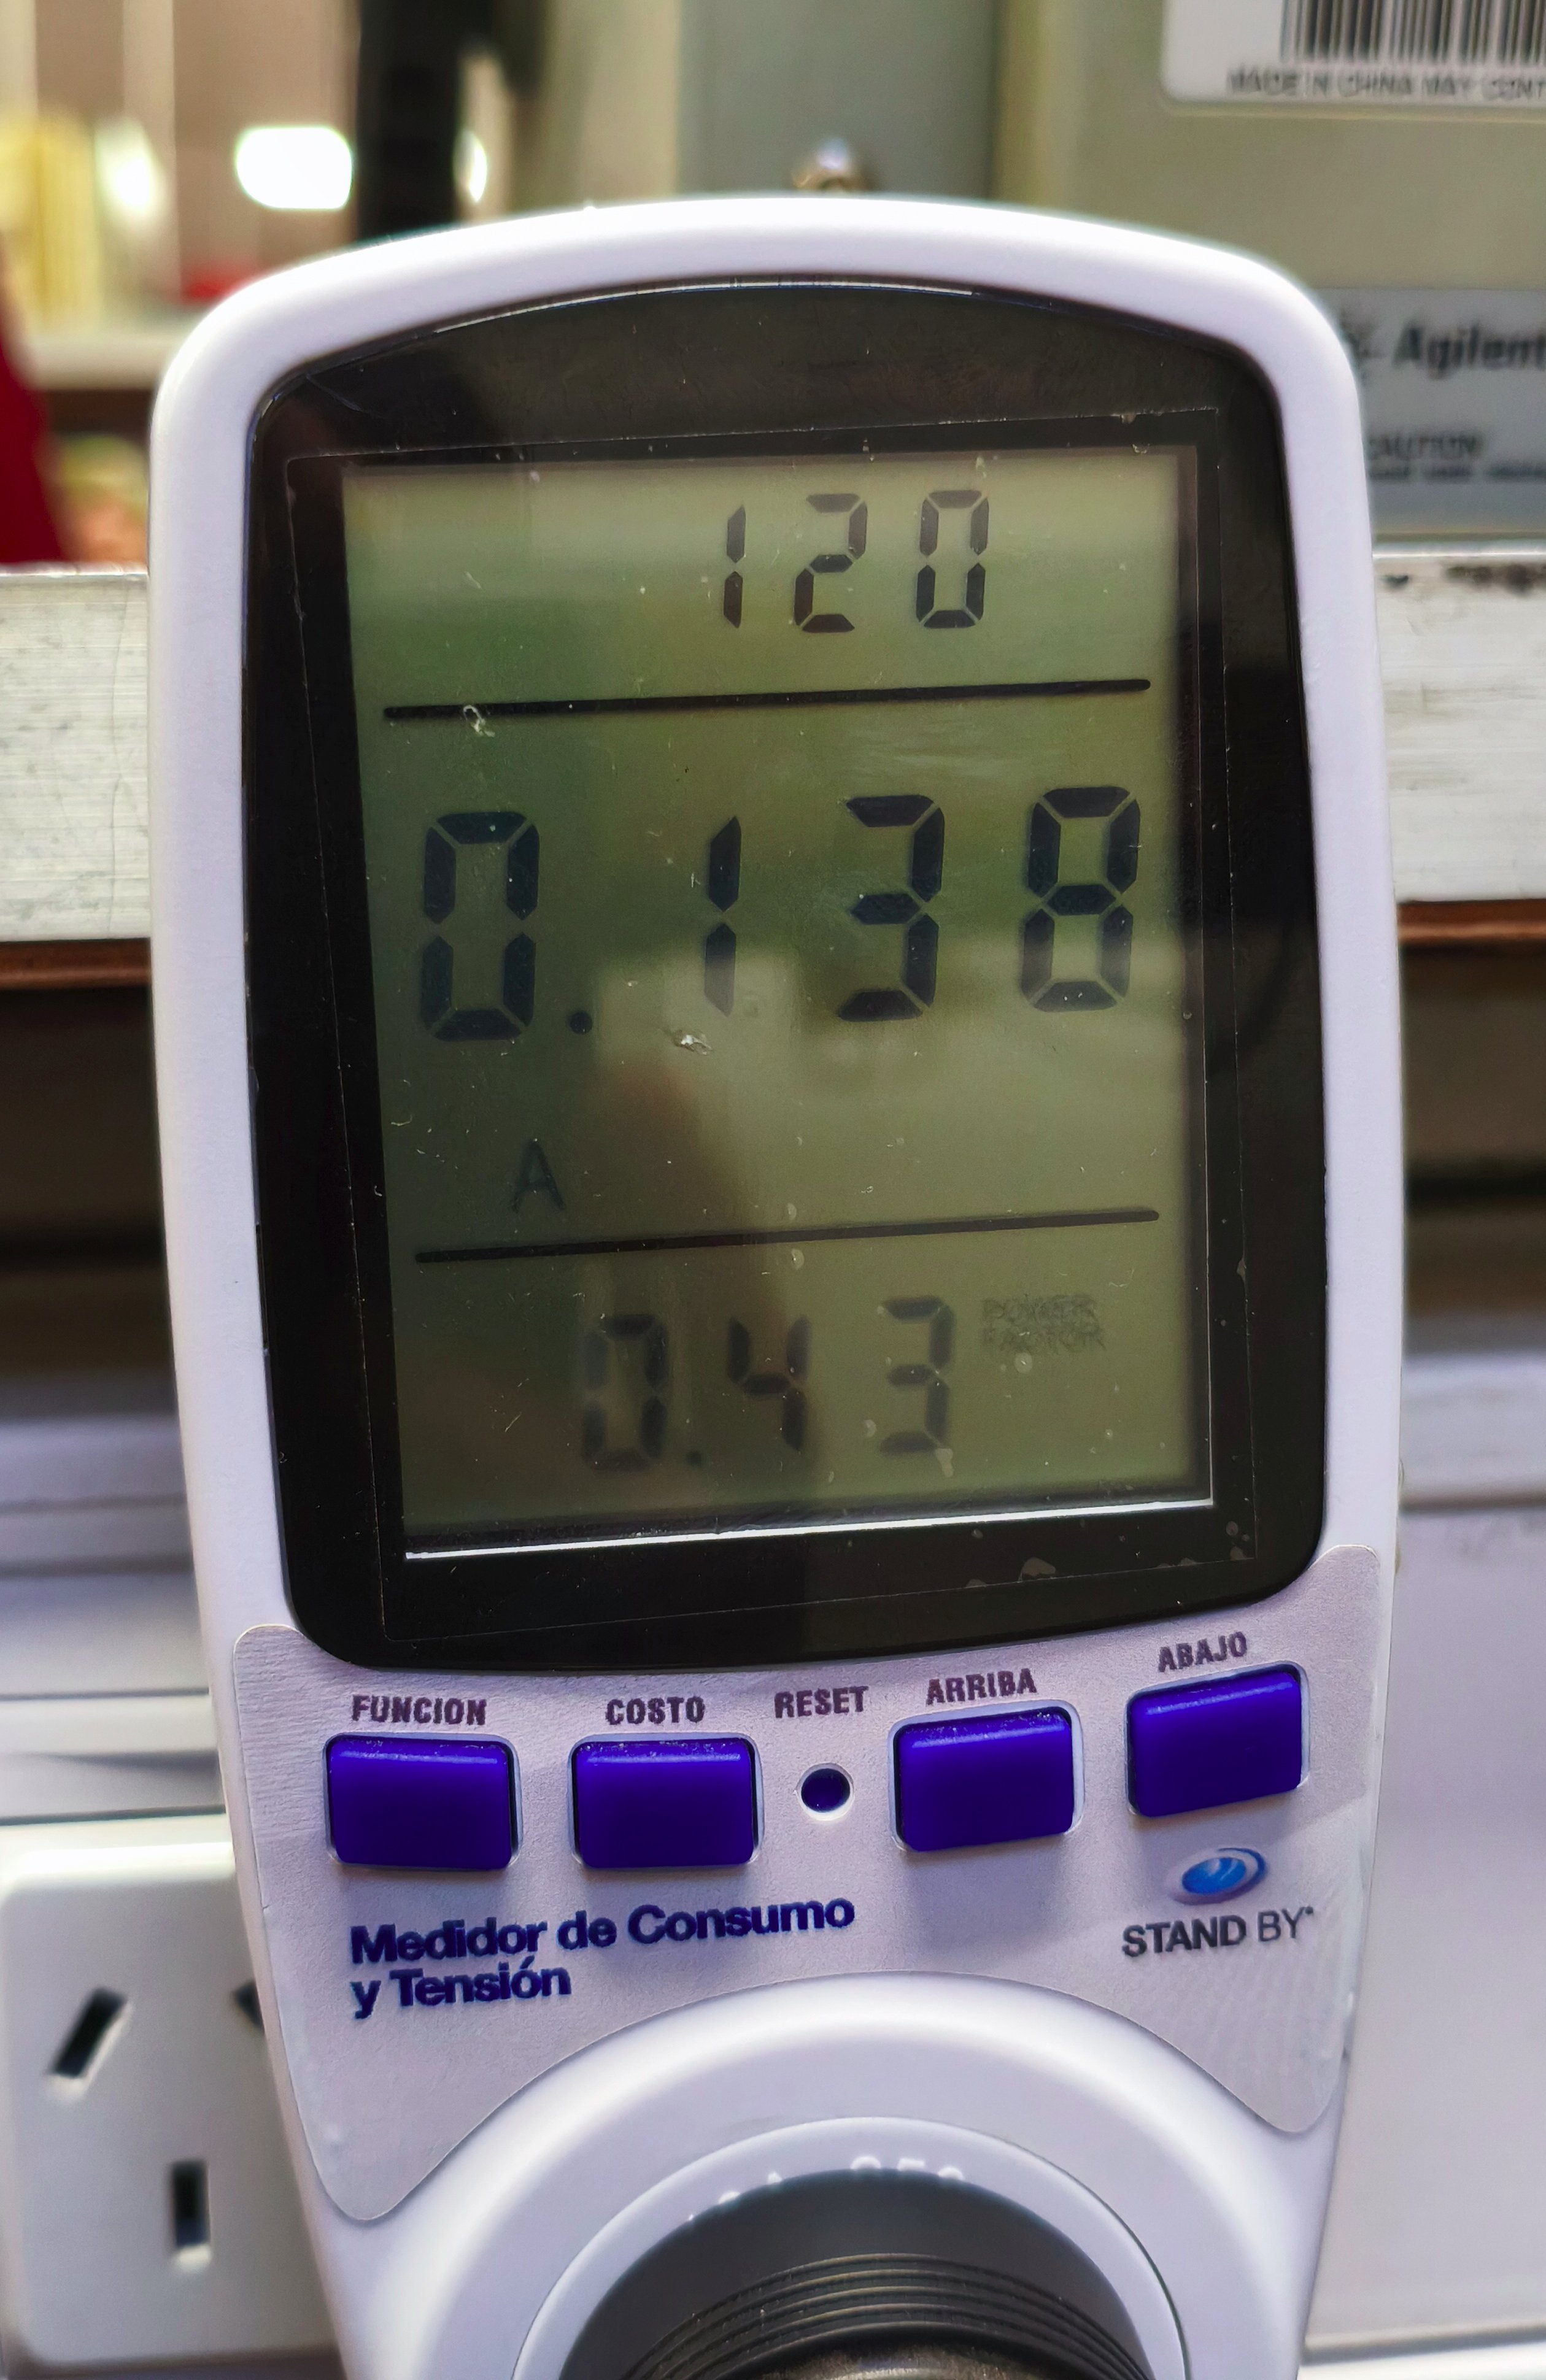
\includegraphics[height=\fotoheight]{pictures/wattmeter.jpg}
        \caption{Lectura en vatímetro digital.}
        \label{fig.dmm:wattmeter}
    \end{subfigure}
    \caption{Montaje de control y medición del factor de potencia con dimmer y carga resistiva.}
    \label{fig.dimmer:setup}
\end{figure}

El desbalance entre la potencia aparente de línea y la potencia activa se debe a la distorsión armónica producida por
la conmutación rápida del Triac, lo cual se desarrollará detalladamente en la sección de conclusiones.
